\chapter{Introduction}
Crystallisation is one of the oldest forms of phase 
separation used by humanity \cite{Schoen1956}, put 
simply, it is the formation and growth of a new 
structured phase within a disordered bulk phase. 
This has applications in a number of industries such 
as pharmaceuticals \cite{Gao2017}, food production 
\cite{Hartel2002}, and electronics \cite{Myerson2002}. 
Where the extraction of dilute materials can help 
improve product quality while keeping production costs 
low. The industrialisation of crystallisation has 
allowed engineers to reliably and efficiently induce 
the crystal formation within a bulk phase. However, 
while on a large scale crystallisation is seemingly an 
understood physical process, just a small amount of 
investigation into the literature reveals that at a 
micro scale there is yet to be unifying theory that can 
accurately explain the process of crystallisation 
\cite{Fu2021}. Crystallisation can be subdivided into 
two steps: Nucleation and Crystal growth. The latter 
focusing on how an already stable crystal grows and how 
it takes on its final shape. Whereas the former is more 
concerned with the first initial moments of a crystals 
formation within a bulk phase.

In this chapter we will outline our current understanding 
of nucleation, why there is a gap in the literature, and why 
there is still a need for local control of nucleation events. 
Furthermore, we will also highlight recent developments 
involving the use of optical tweezers (and other laser based 
methods) in order to develop our understanding of nucleation. 
Lastly we highlight the connection between optical tweezer's 
ability to probe fluid viscosity via rotational motion, and 
the known link between nucleation and fluid flow, to propose 
a novel potential method of creating localised nucleation events.
 
\section{Nucleation}
Nucleation is an example of a binary phase separation, 
where a dilute phase is miscible in a bulk phase, more 
often called the solute and solvent respectively. Because 
of thermodynamics, the two can only remain in equilibrium 
while below a specific concentration ($C_{eq}$) - below 
which the chemical potential $\mu$ for a miscible solution 
is greater than the potential required to separate the two 
phases. Once $C_{eq}$ is exceeded there is a chemical potential 
difference driving the solution to separate the two phases. 
Since different combinations of solute and solvent will 
have different equilibrium concentrations, researchers often 
instead measure the ratio between the solute and solvent by 
using 'supersaturation' \cite{Mullin2001}:
\begin{align}
	\label{eq:supersaturation}
	S(T) = \frac{C_{sol}}{C_{eq}(T)}
\end{align}

Where $C_{sol}$ is just the solute concentration, and 
$C_{eq}(T)$ is the equilibrium concentration at temperature 
$T$. While the solution remains supersaturated there 
is a chemical potential driving the solute to coalesce 
and separate from the solution as an ordered solid, the 
first formation of the crystal is referred to as the 
nucleus and understanding its formation has been the 
focus of researchers for decades now. Typically, for an 
industrial crystallisation process the working principle 
is based on controlling and manipulating the supersaturation 
of the system. 

\subsection{Primary \& Secondary nucleation}
From an industrial perspective, the nucleation process can 
be broadly categorised into either primary of secondary
nucleation. The former describes the formation of an initial
nucleus within the bulk phase, absent of any external stimuli.
Primary nucleation is therefore considered stochastic as there 
is no reliable means of predicting where a nucleus may form, 
or how long it will take. The only reliable indicator being 
that higher supersaturations will result in faster nucleation
rates. At a small scale one can estimate the nucleation rate 
by making repeated measurements of sample solutions and seeing
how many have nucleated after a given time, giving us a Poisson
probability distribution.
\begin{align}
	P(t) = 1 - exp\left[-JV(t-t_g)\right] = \frac{M^*(t)}{M}
\end{align}

Where $J$ is the nucleation rate, $t_g$ is the 'growth time', 
$V$ is the volume of the individual samples, and $M^*(t)$ \& 
$M$ are the number of nucleated samples and the total number 
of samples used respectively. While this is useful for studying
the effects of different parameters at a small scale, for
industrial applications there are to many external factors 
for primary nucleation to be measured accurately. 

Secondary nucleation is the result of a initial seed crystal 
inducing further nucleation within the bulk solution 
\cite{Botsaris1976}. The seed crystals is often specially 
prepared ahead of time and added to a supersaturate solution. 
Due to interactions with the surrounding fluid and the container 
walls it is possible for the seed crystals to act as a surface
for further nucleation \cite{Anwar2015}. Control of secondary 
nucleation events are crucial for ensuring reliable industrial 
crystalliser performance. Fig.~\ref{fig:secondary} depicts an 
attempt of classifying every possible mechanism that could lead 
to secondary nucleation.
\begin{figure}[h!]
	\centering
	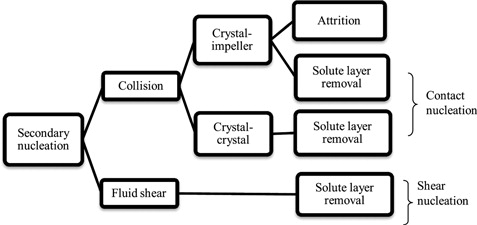
\includegraphics[width=0.95\linewidth]{secondary_nucleation.jpg}
	\caption{Secondary Nucleation mechanisms, classified by
		Agrawal and Paterson \cite{Agrawal2015}}
	\label{fig:secondary}
\end{figure}

This is not a universal classification system, there are a 
variety of opinions on how best to characterise different 
phenomena. It is heavily dependent on the theory used to 
describe nucleation events, this is accurate for both 
secondary and primary nucleation.

\section{Nucleation Theories}
Several potential theories have been proposed to explain 
how nucleation occurs at a microscopic scale. In doing so 
we could potentially predict the expected yield of a given
crystalliser based on the initial conditions of the solution. 
Outlined below are some of the most popular theories currently 
used to describe nucleation. 

\subsection{Classical Nucleation Theory (CNT)}
Sometimes referred to as 'Gibbs Nucleation Theory' the 
original theory was first formed from the works of Volmer 
and Weber, and Frenkel \cite{Frenkel1939, Volmer1926}. 
While initially it was more focused on describing droplet
formation in condensing vapours it was extrapolated to 
describe crystallisation. The central premise of classical 
theory is that nucleation occurs stochastically due to 
collisions between individual solute molecules, ions, or 
atoms. At the same time the bulk phase is resistant to the
formation of a new phase. The competition between these 
random collisions and the bulk solution can be used to 
predict the probability of a newly formed nucleus.
 
Consider a supersaturated solution, after some time 
enough individual sub units collide, forming a nucleus 
of volume $4\pi r^3/3$. The newly formed phase has a 
lower chemical potential than the surrounding solution, 
reducing the free energy of the system. Simultaneously, 
the formation of a new interface is resited by the bulk 
phase due to surface tension. The net free energy of the 
system for a nucleus of radius $r$ is given as \cite{Karthika2016}:
\begin{align}
	\Delta G = \frac{-4\pi r^3}{3v}k_BT\ln(S) + 4\pi r^{2}\sigma_{inf}
	\label{eq:CNT} 
\end{align}

Where $S$ is the supersaturation from eq.~\eqref{eq:supersaturation} 
$v$ is the approximate volume of an individual molecule, 
$k_B$ is the Boltzmann constant, and $\sigma_{inf}$ is the 
interfacial tension of the bulk solution. This assumes that 
the nucleus will have a spherical morphology so that the 
surface tension $\sigma_{inf}$ is a scalar value. Looking at 
\eqref{eq:CNT} suggests that there must be some critical size 
$r$ where the free energy gain from the nucleus exceeds the 
surface tension of the surrounding fluid. This is reflected in 
fig.~\ref{fig:free_energy} where we plot the free energy of the 
system against nucleus size. This reveals a critical size above 
which the gain in free energy exceeds the interfacial tension. 
Furthermore fig.~\ref{fig:free_energy} shows how increasing the 
supersaturation of the system reduces said barrier. 
\begin{figure}[h!]
	\centering
	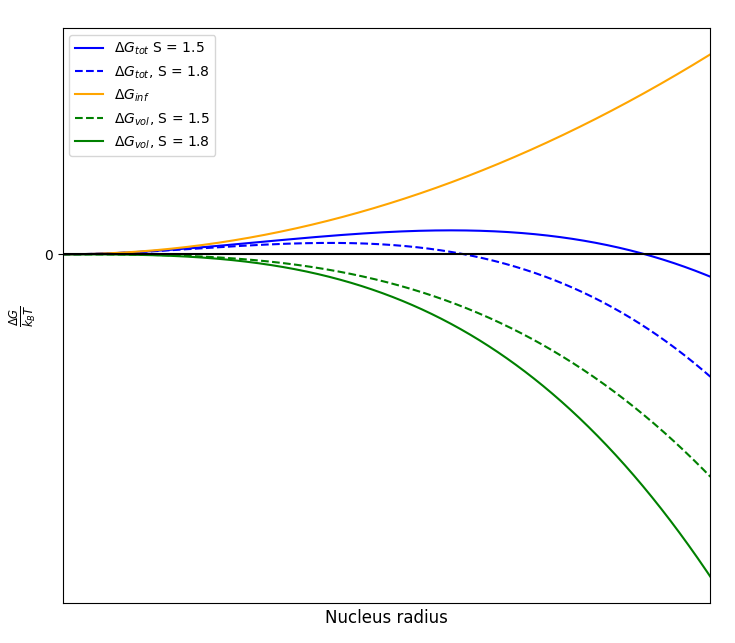
\includegraphics[width=\linewidth]{Free_Energy_Diagram.png}
	\caption{Free energy diagram of a newly formed nucleus according 
		     to the Classical Nucleation Theory. The total free energy (blue)
		     is due to the competition between the volume free energy gain
		     (green) and the interfacial free energy cost (orange). Dotted
		     lines are for a higher supersaturation than the solid lines,
		     the interfacial energy cost is independent of supersaturation.}
	\label{fig:free_energy}
\end{figure}

The maximum value of $\Delta G_{tot}$ is the free energy barrier 
that any newly formed nucleus needs to overcome in order to stabilise. 
The nucleation rate (the volume of new crystalline material formed per 
unit time), is therefore commonly defined as being dependent on the 
energy barrier $\Delta G^*$:
\begin{align}
	J = A \ exp \left[-\frac{\Delta G^*}{k_BT} \right]
\end{align}

Where $A$ is a pre-factor that can be fine tuned to the exact 
demands of the system, the free energy barrier can be found by finding 
the stationary point of $\Delta G_{tot}$. 

CNT is often regarded as a good description of the macro system, its 
obvious that for all crystallization systems there is an inherent energy 
barrier that dictates the nucleation rate. Where it falters is in its 
predictive ability, both in estimating nucleation rates \cite{Gharibeh2005, 
Vekilov2010}, and in the structure of newly formed nuclei \cite{Lee1999, 
Yau2001}. Recent studies suggest classical nucleation is merely one of many 
possible pathways that can be taken to produce a structured crystalline phase. 
Prompting the development of alternative theories to better describe the 
nucleation process.

\subsection{Two Step Nucleation}
The two step nucleation theory is an extension to the CNT 
that suggests that prior to nucleation, the solute will 
form precursor structures. The CNT assumes that solute 
structures below the critical radius should be unstable 
within the solution due to interfacial forces trying to 
dissolve the solute. This assumption is based on the idea 
that any interactions between solute molecules are much
smaller than the surface tension due to the bulk solution.
If instead the solute molecule interactions are significant
then it stands to reason that subcritical liquid-like 
structures are stable. 

The first observation of a liquid-like structure was in 
$CaCO_3$ solutions, initially it was assumed that polymers
were a necessary additive to create a precursor structure 
\cite{Driessche2017, Karthika2016}. This is not the case when 
the solution is above its critical temperature, allowing the 
solution to be in the binodal region of the phase diagram. 
This would result in the formation of two liquid phases, 
one being rich in solute, the other being solute poor 
\cite{Karthika2016, Fu2021}. Several papers later reported 
the presence of stable liquid-like clusters that formed 
prior to nucleation \cite{Savage2009, Wolde1997, Soga1999}. 

\begin{figure}
	\centering
	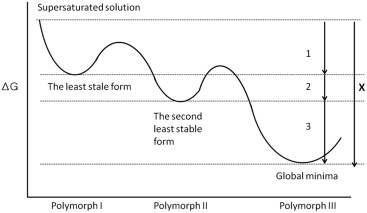
\includegraphics[width=\linewidth]{oswalds_rule.jpg}
	\caption{Free energy diagram of Oswald's rule for a 
	crystal with three possible polymorphs. The diagram 
	shows that there exist local minima in the free energy 
	that represent the different polymorphic forms. A similar
	free energy diagram can be used to describe the two-step
	nucleation mechanism.}
\end{figure}

The formation of these clusters can be understood by Oswald's 
rule; which says that any crystallising system does not 
immediately take the path to the lowest possible energy state 
but instead first transitions to the state with the smallest 
free energy barrier \cite{Ostwald1897}. Oswald's rule was 
assumed to be applicable for crystal polymorphs but can be
generalised to describe the nucleation process also. Further phase 
transitions can still occur but the pathway taken should 
always minimises the overall free energy cost. It is assumed
that between the amorphous phase and the crystalline phase 
the solute undergoes dehydration while changing structurally 
into a more ordered phase, though there is some discussion 
whether the process merely undergoes dehydration, or if there 
is a more complex chemical reaction
\cite{Karthika2016}.

With regards to liquid-precursors, there is still a lot of
discussion about the relationship between the solution 
conditions and the the precursors. The size and rate at 
which these precursors agglomerate based on the degree of 
saturation would provide invaluable information on the 
kinetics of two-step nucleation \cite{Fu2021}. In some 
cases it has even been shown that 'ageing' solutions is 
a necessary step in order to detect the presence of 
stable amorphous clusters \cite{Liao2022}. This was in 
solutions that were supersaturated and yet after the 
formation of precursors spontaneous nucleation was not
seen even after several days of observation \cite{Liao2022}.
This suggests that in some cases the precursors are
metastable and require an external trigger to induce
crystallisation. The presence of metastable structures
and other phenomena has lead to development of a more 
universal theory, namely non-classical nucleation.

\subsection{Non-classical Nucleation} 
Two-step nucleation is based on the idea that between
the bulk solution and the final crystalline phase there
exists and intermediate stage. While this is broadly an
accepted concept, research has shown that in some cases
the intermediate stage can be subdivided into multiple 
states. This has been shown to be the case with metals
in both solid and liquid conditions \cite{Cao2020, Ye2023}
and colloidal simulations have indicated that the 
precursors undergo structural change over time \cite{Tan2013}. 
While in some cases it has been possible to directly
monitor the structural change in the amorphous clusters, 
many organic compounds have not received such treatment
due to the difficulty of characterising and monitoring 
the pre nucleation stage \cite{Fu2021}. This is often 
why two-step nucleation is simply referred to as 
multi-step nucleation. 

There are also a myriad of other unique nucleation events
that deviate significantly from both the classical and 
two-step nucleation theories. A review paper discussing
recent advances in non-classical crystallisation highlighted
that depending on the collision kinetics of the system 
and the molecular interactions could result in drastically
different reaction kinetics. In the former case, unstable
subcritical nuclei have been shown to collide and coalesce
into a supercritical nucleus, but only in conditions where 
subcritical nucleation are plentiful despite a low degree
of supersaturation \cite{Baumgartner2013}. The latter case 
is more prevalent for dipole solute molecules, the anisotropic 
attraction results in nuclei with non-spherical geometries, 
this results in varying kinetics for agglomeration dependent 
on the orientation of each molecule \cite{Yau2001}. Phenomena 
such as the above examples has been collectively refereed to 
as non classical nucleation, it is known that they must be 
related to both CNT and multi-step nucleation but the connection 
is not clear based on the current literature.  

As such, much of the research into nucleation theory is 
focused on developing \textit{in situ} techniques that can 
monitor and characterise the pre nucleation stage, this
would glean information on cases when both classical 
and non-classical nucleation is a possibility 
\cite{Karthika2016}. 

%%%%%%%%%%%%%%%%%%%%%%%%%%%%%%%%%%%%%%%%%%%%%%%%%%%%%%%%%%%%%%%%%%%%%%%%%%%%%
\section{In situ techniques for studying nucleation}
There are several different phenomena \cite{Fu2021, Karthika2016} 
that are not well described by any individual theoretical framework 
(CNT or multi-step nucleation for example). There is an increasing 
interest in probing the pre-nucleated solution.

One of the key conclusions is the need for the development of 
better \textit{in situ} techniques for characterizing and 
imaging the nucleation pathways. Understanding which specific 
pathway is unfolding under a certain set of experimental 
parameters would allow one to develop a map of the thermodynamic 
landscape available to a pre-nucleation system. The challenge 
therein lies in developing experimental methods by which one can 
reproduce similar nucleation events and in turn use 
characterisation techniques to identify the pathway taken. The 
method not only needs to be repeatable fora single set of system 
parameters, but also needs to be flexible enough to replicate 
results regardless of the system parameters (i.e. varying 
supersaturation, temperature, and solute choice). There have 
been several different methods deployed to try and observe 
crystallisation at a microscopic scale.

\subsection{Computer Simulations}
While not a direct observation of nucleation events, computer
simulations have proved an invaluable tool for studying and 
testing predictions about the pre-nucleated solution. By 
comparing the simulative nucleation rate to the expected 
rate given by current models, researchers can test newly 
developed theories and glean information about the microscopic
parameters of a system. 

The main challenge facing computer simulations is the issue
of limited scope. Molecular dynamic simulations are constrained
by their choice of time and length scale, for example simulations
in a canonical ensemble face issues where the chemical potential
is depleted to the point that the driving force for crystallisation
is halted \cite{DuranOlivencia2015, Finney2023}, this can be 
addressed but requires an extensive increase in computational 
resources to maintain the chemical potential equilibria. Like wise
in most cases the choice of time scale is a crucial factor, shorter
time scales provide a more accurate evolution of the solution; 
however, in some cases the time scale magnitude for crystallisation
is often far greater than the time scale used in the simulation. This
has led to more advanced sampling techniques that allow for longer 
time scales which has provided insights into the pre-nucleation 
solution stage and formation of pre-nucleated clusters \cite{Finney2023}.
 
The study of the pre-nucleated solution and the evolution of 
precursors has been aided greatly by the use of simulative 
studies. Early on it was shown in colloidal crystallisation 
that the structure of the precursor was time dependent; 
colloidal simulations showed that regardless of the molecular
interactions between colloids the atomic packing pattern was 
predominately hexagonal centred, over time the packing
became dominated by body centred packing in the case 
where the interactions were longer reaching \cite{Tan2013}. 
They also confirmed that precursor formation was driven not
by local density variations, but instead was driven by the 
local bond order of the colloidal precursors \cite{Tan2013}, 
providing strong evidence that the colloidal pre-nucleation 
clusters undergo rearrangement prior to nucleation. Further
developments in $NaCl$ simulations have shown that by varying
the density fluctuations the precursor structure could either
be amorphous, the classical rock-salt structure, or a new 
structure similar to wurtzite. While this result is difficult
to confirm it provides a important conclusion, that simulations
can hint at new nucleation pathways that have not been confirmed
experimentally. This means that computer simulations can not
be merely used to confirm theories, but can be used to examine
and search for novel results. 

Overall computer simulations make up a core area of research 
in the study of nucleation. The technique is however limited,
often struggling to examine nucleation over longer time scales
or larger number of particles. While sampling methods and 
enhanced simulation techniques has alleviated this somewhat 
they are still far from being able to describe the behaviour 
of larger molecules undergoing nucleation. 


\subsection{Transmission Electron Microscope (TEM)}
One of the more well known techniques used for direct observations 
of crystallisation dynamics is using transmission electron 
microscopy (TEM). The basic working principle involves creating a 
focused beam of electrons that are directed onto a target sample.
Due to the wave-particle duality, the electrons can be treated 
as a unified beam of light, whose wavelength is dependent on the 
kinetic energy of the electrons. The wavelength of an individual 
electron is given by \cite{Williams2009}:
\begin{align}
	\lambda_e = \frac{h}{\sqrt{2mE(1+\frac{E}{2mc^2})}}
\end{align}

\noindent
When incident on a sample the wave is scattered by the sample 
and can then be detected by an imaging screen that measures 
the difference in intensity between the scattered and 
transmitted beams. The advantage of TEM is that one can bypass
the diffraction limit imposed by visible light, the maximum 
resolution that can be achieved by a microscope is given by
\cite{Champness2020}:
\begin{align}
	d = \frac{\lambda}{2NA}
\end{align} 

\noindent
where NA is the numerical aperture of the objective lens, and
$\lambda$ is the wavelength of light used to illuminate a sample.
For a visible light LED with an average wavelength of $550~nm$, 
the upper limit for an objective lens (NA of 1.2) is around 
$230~nm$ whereas a similar lens focusing an electron beam 
with an average kinetic energy of $100~keV$ will have a maximum 
resolution of just over $4~pm$ \cite{Champness2020}. There is
an upper limit to the maximum resolution possible as electron 
lens are far inferior to what modern optics can achieve 
\cite{Champness2020} so there is a trade off between quality and 
resolution. 

TEM technology has proven invaluable to the study of nucleation
at an atomic level. The samples are often only a few hundred 
atoms thick in order to optimise the imaging results. Much of 
the supporting evidence for non-classical nucleation has been 
demonstrated via TEM \cite{Ye2023}. For example when Cao 
\textit{et al} observed the formation of amorphous atomic 
cluster using $\gamma-$Fe,Au, and Re; all three of which 
underwent continuous transformation before eventually 
reaching an final ordered state \cite{Cao2020}. The amorphous 
cluster did not immediately transition to an ordered structure, 
instead fluctuating somewhat randomly until eventually settling 
into a crystalline structure \cite{Cao2020}. This was confirmed 
both in solid growth and liquid growth conditions \cite{Cao2020, 
Loh2016}, suggesting that the non-classical nucleation path 
dominates in all cases of metal crystal formation \cite{Ye2023}. 
Confirmation is necessary for different solute choices, as in 
the case of organic solids it is believed that non-classical 
nucleation only dominates in low supersaturations whereas 
classical nucleation is dominate at higher supersaturations.

TEM analysis has not been extended to the study of organic 
crystals, proteins, or simple salts at an atomic level 
however. The main reason being that organic materials can be 
damaged by the electron beam and therefore need to be frozen 
prior to being imaged \cite{Champness2020}. This was used to 
study the polymorphic time dependence of glycine crystals, by 
varying the time prior to freezing Broadhurst \textit{et al} 
showed that $\beta$ glycine dominates initially but $\alpha$-
glycine is more stable after a longer period, $\gamma$-glycine 
was only found when allowed to dry over an hour on a glass slide \cite{Broadhurst2020}. While this was invaluable for showing 
the time scales with which polymorphs form, it doesn't provide 
much information on the kinetics of crystal growth as these 
were snap shots and not direct observations of the nucleation 
process.

Overall TEM analysis is invaluable for the study of atomic 
crystal growth, the secondary scattering from electron 
beams also allows for chemical and structural information 
to be gleaned from the target. This has given strong evidence
for the non-classical nucleation theory, particularly in 
metal crystal formation. Due to the high energy of the 
electrons, organic materials have not received the same
focus outside of cryoTEM analysis. Non-invasive methods
are therefore necessary to gain an understanding of the
crystal growth and formation of organic crystals, 
particularly when both classical and multi-step nucleation 
can occur.


\section{Optical Tweezers}
\subsection{Background}
Optical tweezing has been a field of applied optics ever since 
the 1980s when Ashkin \cite{Ashkin1970} first showed that focused 
light was capable of trapping micron sized particles due to light 
exerting 'radiation pressure'. The working principle was that a 
light source such as a laser could trap small objects within a 2D 
plane, as long as the light source had an approximately Gaussian 
profile (colloquially called a Gaussian beam). Soon after, Ashkin 
showed that the introduction of a microscope objective would allow 
one to focus the light source to a diffraction limited point that 
would stably trap small objects within a confined volume 
\cite{Ashkin1980}. This allowed Ashkin and others to study individual 
biological cells as the overall force was on the order of $10^{-12}\ 
N$ while being non-invasive to the internal structure. Later it would 
be used to probe microscopic properties such as the formation of 
colloidal aggregates \cite{Yi2021} to the drag forces exerted by a 
pure vacuum \cite{Ahn2018, Monteiro2018}. Due to the predictable 
behaviour of light, optical tweezers have become essential for 
measuring and exerting precise forces on the magnitude of pico-newtons 
allowing one to probe the material properties of the smallest 
materials. 

\subsection{Literature related to laser induced nucleation}
From as early as 1996 it has been known that laser irradiation 
using a Gaussian beam is a viable method of inducing nucleation 
within a supersaturated solution \cite{Garetz1996}. The first 
reported case was notable as it used a 1.064 $\mu m$ laser, the 
glycine solutions would appear transparent to such a laser which 
would suggest there was no photo-chemical reaction. Later studies 
into this phenomena found that the laser polarisation can influence 
the polymorph produced. With circularly polarised light producing 
$\alpha$-glycine and linearly polarised light forming $\gamma$-glycine 
\cite{Garetz2002}. Future research has found nucleation can be 
induced by 1 of 3 routes.

\subsubsection{Non-Photochemical Laser Induced Nucleation}
Non-photochemical laser induced nucleation (NPLIN) involves 
irradiating a solution with a pulsed laser \cite{Garetz1996,
Garetz2002,Sun2006}. The laser itself does not have to be 
heavily focused, instead irradiating a large region of the 
solution all at once. The choice of laser is of particular 
importance; with nucleation probability changing depending 
on the wavelength. A study of KCl solutions found that for 
lower intensities it was found that nucleation was favoured 
for lower wavelengths but above a peak intensity of $5 MW/
cm^2$ the wavelength independence disappeared \cite{Kacker2017}. 
Measurements of the intensity prior and after irradiation 
confirmed this wavelength dependence was not due to any 
photo-chemical interactions \cite{Kacker2017}.

Additionally, the choice of solute will effect the setup, not 
only because some solute's are unaffected, but also because 
there is a minimum laser threshold before nucleation is observed 
\cite{Garetz2002}. Several papers have debated the exact mechanism 
that induces NPLIN \cite{Garetz2002, Knott2011}. A suggested 
theory to this is an optical Kerr effect: For anisotropically 
charged solute molecules the electric field can reorient them 
to match the propagation direction \cite{Garetz2002}. If enough 
molecules are co-aligned the free energy barrier is reduced to 
allow for ambient nucleation \cite{Knott2011}. An alternative 
theory is the dielectric polarisation effect, in conditions that 
are unfavourable to cluster formation the polarising effect can 
stabilise the clusters \cite{Alexander2008}. As the cluster 
concentration rises so does the likelihood of nucleation 
\cite{Vekilov2010}. 

Both theories are similar to one another but where the optical 
Kerr theory is limited to anisotropic solute molecules, the 
direct polarisation theory is more flexible. Regardless both 
theories struggle to explain why the phenomena is not observed 
in all nucleation systems \cite{Korede2023}, such as acetamide 
which is similar to urea which does nucleate when irradiated 
\cite{Ward2016}. One of the benefits of NPLIN is that since the 
pulses are relatively low in their intensity they can be fired 
off quickly in succession, allowing for continuos crystallisation 
set ups. Overall, the NPLIN phenomena needs further research to 
properly describe its effects. The mean pulse intensity needs to 
be kept relatively low (on the order of $0.1-0.01 GW/cm^2$), as 
high intensity pulses lead to a completely different nucleation 
mechanism.

\subsubsection{High Intensity Laser Induced Nucleation}
High intensity laser induced nucleation (HILIN), where the pulse 
intensity is on the order of several $PW/cm^2$ is far simpler a 
mechanism to explain in comparison to NPLIN. The production of 
nuclei can be wholly associated to a cavitation process within 
the target solution, where the laser focus results in thermo-
cavitation and the subsequent pressure wave leads to a nucleation 
event around the focus of the laser \cite{Yoshikawa2005, Soare2011, 
Barber2019}. 

What remains in question is both how the physical properties (size, 
polymorph, etc) are influenced by the cavitation process, and how 
the pressure change triggers nucleation. The former has already 
been investigated; by adjusting the focal position Ikeda \textit{et 
al} could control the polymorph of indomethacin \cite{Ikeda2015}, 
this is not a universal method however, as it has also been shown 
that laser power can influence the crystal polymorph \cite{Wang2010}. 
The latter is a tricky task to address due to the fact that these 
cavitation bubbles form and collapse in less than $100\ \mu s$. 
Using fluorescence dyed proteins, researchers were able to observe 
a sudden spike in fluorescence just as the cavitation bubble began 
to collapse, they suggested that due to the collapse of the cavitation 
bubble the protein clusters are brought together at the lasers focal 
point. However, while the fluorescence imaging indicates a local 
concentration increase it is difficult to quantify this change 
depending on the size of the bubble \cite{Korede2023}. It has been 
suggested that in theory any solution can undergo HILIN 
\cite{Korede2023}, but proving such a theory requires a clear 
understanding of the phenomena both before and after cavitation occurs. 
Current research aims to combine experimental research with computer 
simulations to develop a universal theory, with the hope that this 
could also be related to NPLIN.   

\subsubsection{Trapping Induced Nucleation}
Lastly, there is trapping induced nucleation, this is where optical 
tweezers come into play. Due to the radiation pressure created by 
the focused beam, it is possible to manipulate the solute, this was 
demonstrated with amino acids such as glycine \cite{Tsuboi2009}. 
Whether or not a crystal forms is due to the location of the laser 
focus. When focusing on the cover slip, supersaturated solutions 
of glycine and $D_2O$ were shown to create a dense liquid droplet 
of glycine and water \cite{Yuyama2010, Yuyama2012}. The dipole 
moment of the glycine molecules is too small to be influenced by 
the optical trap, as such it would suggest that larger aggregates 
are being manipulated. Applying DLS analysis to the dense liquid 
region showed that it was populated by clusters that would 
consolidate together upon being focused by the optical trap 
\cite{Gowayed2021}. Molecular simulations of glycine solutions 
showed that these clusters are unstable when using pure glycine 
below the saturation point suggesting that the clusters are 
formed due to glycine reaction products \cite{Sweatman2022}. 
When the optical trap is moved from the cover slip to the 
air-solution interface, nucleation would occur before a dense 
liquid region could form \cite{Yuyama2010}. Repeated experiments 
where the laser is focused on the air-solution interface have 
lead to a variety of different nucleation events. In some 
instances the nucleation occurs spontaneously after a short 
period of time \cite{Yuyama2010}. Whereas allowing a solution to 
age results in the formation of amorphous precursors that when 
irradiated will nucleate immediately \cite{Liao2022}. The 
precursors are only seen when the solution is irradiated by an 
optical tweezer and the growth rate can be controlled somewhat 
by varying the laser power \cite{Liao2022}. The reason why 
nucleation is only seen at the air-solution interface is due 
to the limited molecular mobility close to the interface. 
Often tweezing experiments will use a hydrophilic coating to 
minimise the height of the solution droplet and further limit
the molecular mobility \cite{Yuyama2012, Gowayed2021}.

Walton and Wynne discussed a plausible model for how the tweezer 
focus could result in a nucleation event. Put simply, when the 
laser is focused at the solution the radiation pressure draws 
in solute material, creating a concentrated region of solute. 
This also creates a depleted region around the focus and raises 
the local temperature. When the laser is turned off the depleted 
region around the focus quickly cools back to the ambient 
temperature. This sudden cooling allows for nucleation to occur
just outside the focus.  

Laser induced nucleation has the potential to be a viable method 
for \textit{in-situ} studying of nucleation events. Using high 
numerical aperture lens one can localise the nucleation event 
to a specific region of the solution. The current issue is that 
the mechanism behind laser induced nucleation is not fully 
understood, as such it is rather difficult to modify the laser 
for different solution parameters. Instead it may be more 
effective to manipulate the solution using trapped particles. 
One way would to generate an optical torque on a trapped particle
and therefore shear the surrounding fluid, a method that is 
already in common use for micro-rheological studies \cite{Bishop2004, 
RobertsonAnderson2018}

\subsection{Optical Torque and rotation}
\label{sec:opt_torque}
It has long been known that electromagnetic fields can transfer
linear and angular momentum \cite{Beth1936MechanicalDA}; more 
accurately the field is said to have both orbital and spin momentum. 
Though there is some debate on how to decompose the total momentum 
into these two components \cite{Bruce2020, Svak2018}, for this 
project we do not need to calculate the exact quantities and will 
instead look at the broader effects of both components. Orbital 
angular momentum arises from the shape of the wavefront of the 
particular field in question; for simple Gaussian beams the wavefronts 
are uniform and equally spaced resulting in the typical radiation 
pressure that Ashkin and co demonstrated \cite{Ashkin1980}. However, 
higher order modes of a Gaussian beam (for example: Laguerre-Gaussian 
modes) have non-uniform wave fronts meaning the orbital momentum has 
both angular and linear components; depending on the relative size 
of the target particle one can induce rotation, or orbiting 
\cite{Bruce2020, Courtial2000}. 

Spin angular momentum (SAM) is attributed to the spin density of 
the field, early research has shown that the spin density is non-
zero for any beam despite the fact that the total SAM transferred 
to a medium is 0 \cite{Svak2018, Bliokh2014}. This has sparked 
debate if SAM is even a physical quantity as it does not aid in 
the transport of energy directly \cite{Bliokh2014} and so cannot 
be directly observed in some cases despite being non-zero. This 
paradox is resolved by representing the wave as an array of spin 
momentum loops that cancel one-another out when the medium is 
homogeneous.Spacial inhomogeneities cause these spin loops to no 
longer be equal, resulting in non-zero spin density, anisotropic 
mediums (such as birefringent crystal lattices) experience a 
transfer of spin angular momentum, imparting an optical torque.

Birefringence is a material property often seen in crystalline 
materials, where the crystal lattice has a different structure 
dependent on its orientation. Since light is composed of waves 
that propagate in orthogonally to one another, a birefringent 
material will refract light differently depending on the light's 
polarisation. Therefore it can be said that the material has 
two separate refractive indices. For circularly polarised light 
this inhomogeneity results in a high degree of SAM being 
transferred to the target object \cite{Parkin2009, Arita2016}. 
The greater the difference between the two refractive indices the 
greater the angular momentum transfer.

The ability to transfer angular momentum has been exploited 
to rotate microspheres as fast as 1000 Hz while suspended 
in a bulk medium \cite{Arita2016} as well as a means of 
measuring the local temperature and shear response of said 
medium \cite{Millen2014, RodriguezSevilla2018}. Calculating 
the optical torque applied to a birefringent material is given 
via:
\begin{equation}
	\label{eq:opt_torque}
	\begin{aligned}
		\tau_{opt} =& -\frac{\epsilon}{2\omega_{laser}}E_0^2sin(kd(\Delta n))cos2\theta sin2\phi 
		\\ &+  \frac{\epsilon}{2\omega_{laser}}E_0^2 (1-cos(kd(\Delta n))sin2\phi)
	\end{aligned}
\end{equation}

Where $\Delta n$ is the difference between the two refractive 
indices, $\theta$ is the angle between the particle's long 
axis and the polarisation vector of the local EM field, and 
$\phi$ is the phase shift in the EM field. The first term 
represents the 'orientational' torque which aligns the long 
axis of the particle with the electric field, when aligned 
$\theta=0$ meaning the entire term is negligible for particle's 
with a stable orientation. The second term is due purely to the 
polarisation of the laser, for circularly polarised light 
$\phi=\pi/4$ thus maximising the torque transferred to the 
target particle. Eq.~\eqref{eq:opt_torque} is only applicable 
for particles with a known birefringence, but there are other 
mechanisms that result in optical torque.

A common example is shape induced birefringence. If a particle 
has an anisotropic shape, it is more susceptible to being 
polarised along its longer axis than its shorter axis. Consider, 
for example, an ellipsoid elongated along one of its primary 
axis' ($r_z > r_x = r_y$). In a plane polarised beam such a 
particle will align with the polarisation vector. Therefore, 
the particle will rotate as angular momentum is transferred 
along its long axis. One common feature, regardless of shape,
is that a particle with shape birefringence will rotate when 
it lies perpendicular to the direction of propagation. This 
is seen most evidently with spherical dimers \cite{Ahn2018, 
Reimann2018} but even for elliptical particles rotational 
motion is only detected when their long axis is not aligned 
with the direction of propagation \cite{Zhu2021, Mihiretie2014}.

Often the optical torque experienced is far greater than similar 
spherical particles that are birefringent \cite{Bruce2020}. 
Currently spherical dimers are being rotated in vacuums to 
measure quantum forces and torques \cite{Ahn2018, Reimann2018}. 
There are some alternative cases where particles are rotated 
while not being aligned in the plane of the polarisation. However 
in these cases their shape is often specifically engineered to 
scatter light in such a way that the net momentum change always
occurs in one direction regardless of the laser polarisation 
\cite{Higurashi1994}. 

Other examples of optical torque is when an anisotropic 
particle is aligned with the beam's direction of propagation 
(in which case $\theta=\pi/2$ and the first term disappears). 
This is analogous to an optically trapped sphere, where 
alongside a restoring force the particle also experiences a 
restoring torque. This seemingly random rotational motion is 
referred to as libation \cite{Bruce2020},often in typical 
suspension trapping situations (where the particle is suspended 
in a fluid) the rotational motion is washed out by the 
translational motion. As such, many experiments elect to trap 
in low pressure environments to precisely measure the optical 
torque being exerted by the optical trap \cite{Ahn2018}. This 
has lead experiments to try and achieve '0 kelvin' motion, 
where by trapping a silica dimer they were able to restrict its 
motion using 3 optical traps simultaneously. Despite this, they 
found that the dimer's rotational motion about its long axis 
could not be controlled leading to the undesired rotational
modes \cite{Bang2020}.

The detection and measurement of optical torque is still a 
field of intense research, not only does it have potential 
to understand quantum fluctuations in a particle's motion 
but also allows for the creation of more effective
micro-rotors. The latter being especially pertinent for 
understanding the behaviour of fluids experiencing localised 
shearing.

\subsection{Characterisation of rotational motion}

Rotational motion about a single axis is easiest to account for.  
When the power spectra of elliptical polystyrene particles was 
fitted by Yogesh \textit{et al} \cite{Yogesha2011PreciseCO}, they 
assumed that the rotational motion was purely in the transverse
plane. As such they did not have to account for any variance in 
the trapping strength due to orientation nor did they need to
consider non-periodic rotational behaviour. In the case where 
rotational motion is stochastic the problem is more complex. 
For example, when an optical fibre trap characterisation 
technique was implemented by Saffron \textit{et al} 
\cite{BarZiv1997, Meller1998}, they were able to use dynamic 
light scattering to characterise both the axial and lateral 
trap stiffness acting on microspheres. The only drawback 
admitted to in their work was that the technique was constrained 
to isotropic scatters as their theoretical model for describing 
the auto-correlation function was predicated on the fact that 
any variations in the signal are due to the particles 
translational motion within the confines of a cylindrical trap 
\cite{BarZiv1997}. Where the upper limit of the cylindrical 
trap is given by the Rayleigh range ($z_R = n\omega_0/NA$).
However, as demonstrated by the results from Chapter 4.1, 
the axial traps of spherical aggregates is often situated 
far beyond the Rayleigh range (for a 1.2 NA laser this is 
$\pm5.985 \mu m$).

\section{Shear induced Nucleation}
It has long been known that fluid shear rate plays a role in 
influencing nucleation; however, the exact relationship between 
shear rate and nucleation rate has only been recently understood 
for specific solutions. Theoretical research into shear induced 
nucleation suggests that there should be a slight increase in the 
nucleation rate at low shear rates, reaching a maximum increase in 
nucleation rate, and then at higher shear rates the nucleation rate 
begins to drop off. 

This has been shown theoretically for both simple colloidal 
\cite{Mura2016,Debuysschere2023,Richard2015} and ice crystal 
formation \cite{Goswami2020}; however, no experimental work 
into these systems has been conducted to confirm these theories. 
There is some experimental evidence for this phenomena in simple 
salt and protein solutions - though the authors emphasise that 
mechanical agitation cannot be ruled out - there has not been a 
exhaustive study into the shearing effects apart from in glycine 
solutions. In \cite{Debuysschere2023} it was found that a shear 
rate of around $3000\ s^{-1}$ was the maximum shear rate that 
would yield the highest nucleation rate. Using the theoretical 
model established in \cite{Mura2016,2001} which modifies the CNT 
to account for the effects of a nucleus undergoing shearing, 
accounting for the fact that a nucleus' growth is undergoing 
competition between flow-mediated molecular transport and the 
strain applied by the flow field which inhibits the growth of 
the nucleus. There central conclusion (from both the theoretical 
and experimental results) is that there is an optimal shear rate 
in which the nucleation rate is maximised. 

However, a question that arises from this result, if there is 
a optimal shear rate in which molecular transport is maximised 
and strain is minimised, then surely there should also be a shear 
rate in which the molecular transport and strain are equal - 
allowing one to suspend a nucleus at a constant radius. In this 
scenario, the molecular transport would prevent the nucleus from 
dissolving, but the strain would prevent the nucleus from growing. 
This however would require one to be able to apply a continuous 
shear rate to a targeted nucleus with high precision, there is 
also no model for an individual nucleus in a continuous fluid 
field. 

\section{Significance of Thesis}
As I have hoped to make clear in the above introduction, the 
current state of nucleation theory is rather cumbersome at a 
micro-level. Models such as CNT and multi-step nucleation are 
not sufficient for describing the myriad of potential pathways 
nucleation can go down. As suggested by some review articles, 
the best way to address this is by developing \textit{in-situ} 
methods that can study the pre nucleation phase in greater detail 
\cite{Fu2021}. Furthermore, the ability to localise nucleation 
allows for better characterisation of the kinetics of crystal 
growth. Laser induced nucleation stands to be an ideal method to 
study nucleation, as the laser output can be concentrated to a 
small area \cite{Korede2023}. This fine control over the local 
fluid would allow for individual nucleation events to be
characterised as a factor of the local fluid properties. One 
challenge lies in the fact that its clear that the local fluid 
properties have a direct influence on the likelihood of laser
induced nucleation from occurring \cite{Korede2023, Ward2016,
Yuyama2012, Liao2022}. 

A way around this would be to try and induce the local fluid 
without directly relying on the electromagnetic field. Optical 
tweezers can reliably do so already by applying an optical 
torque to a trapped particle in order to induce fluid flow 
\cite{Bishop2004, RobertsonAnderson2018}. It's already well
documented that shearing will enhance nucleation events at a
macro-level \cite{Debuysschere2023}. Micro-rheological studies 
using optical tweezing have been more interested in probing 
the local viscosity rather than try and use it as a means of 
shearing the fluid to induce crystal growth. 

\section{Overview}
Overall the aim of the PhD is to study viability of using 
micro-rotors to generate localised fluid flow around the 
beam focus. The results are reported in chapter 3, this is 
then followed by experimental work where we use a galvano-
mirror to move the beam and hence generate shear flow. While 
overall unsuccessful the addition of a moving beam focus 
showed that the growth of a nucleus can be localised around 
the trap focus. This presents a new insights for controlling 
and studying the growth of a newly formed nucleus by precise 
movement of the trapping focus.

The latter chapters cover computer simulations into the 
behaviour of microscopic spherical dimers in an optical
trap. Prior research into dimers using back focal plane
interferometry has mostly considered their trapping 
behaviour to be similar to a single sphere but with a 
difference in trapping strength. Computer simulations
reveal a host of new behaviours dependent on the dimer's
size, orientation, proximity to the trapping focus, and 
even the polarisation of the trapping beam. The latter in
particular suggests that multi-spherical particles can act
as sophisticated micro-rotors. 

However, this raises a its own host of experimental challenges,
namely how do we characterise the behaviour of an arbitrary
particle. Relying on current characterisation techniques is not
possible as they are predicated on the trapping object to behave
like an isolated sphere. Two novel methods of measuring rotational 
motion are discussed in chapter 5; firstly via a novel detection 
fibre method that allows for instantaneous measurements of the 
orientational behaviour of optically trapped ellipsoids/dimers; 
and secondly we create a simulative quadrant photo diode that 
replicates laboratory results, utilising linear regression 
techniques we measure the change in orientation in order to 
measure the optical torque applied to a non-birefringent particle. 
